\documentclass{beamer}
\usepackage[utf8]{inputenc}

\usepackage{amsmath}
\usepackage{graphicx}
\usepackage{url}
\usepackage{fancyvrb}
\usepackage{xcolor}

\usetheme{Boadilla}
\usecolortheme{whale}
\usepackage{lmodern}

\usepackage{listings}

\mode<presentation>

\definecolor{orange}{HTML}{BC2E07}

\usepackage{hyperref}
\hypersetup{
    colorlinks,
    linkcolor=orange,
    urlcolor=blue
}

\title{Lab \# 0: Yak Shaving}
\subtitle{EC-102 -- Computer Systems and Programming}

\author{Usman Ayub Sheikh}
\institute{School of Mechanical and Manufacturing Engineering (SMME), \\ National University of Sciences and Technology (NUST)}
\date{\today}

\begin{document}
\begin{frame}
    \titlepage
\end{frame}

\begin{frame}
    \frametitle{Outline}
    \begin{columns}
        \column{0.5\textwidth}
        \tableofcontents
        \column{0.5\textwidth}
        \begin{figure}
            \centering
            
\includegraphics[scale=0.26]{yak-shaving}
        \end{figure}
        Any \emph{apparently} useless activity which, by allowing you to overcome intermediate difficulties, allows you to solve a larger problem.
    \end{columns}
\end{frame}

\begin{frame}
    \frametitle{What is IDE?}
    \section{Setting Up Integrated Development Environment} % (fold)
    \label{sec:setting_up_development_environment}
    \subsection{What is IDE?} % (fold)
    \label{sub:what_is_ide}
    A programming environment packaged as an application program, typically consisting of
    \begin{itemize}
        \item a code editor,
        \item a compiler,
        \item a debugger, and
        \item a graphical user interface (GUI) builder.
    \end{itemize}
\end{frame}

\begin{frame}
    \frametitle{Downloading Setup Files}
    \subsection{Downloading Setup Files} % (fold)
    \label{sub:downloading_setup_files}
    Step \# 1: Download Visual Studio 2010 Professional/Ultimate from \href{http://stackoverflow.com/questions/8894654/vs-2010-trial-version-link}{here}.
    \begin{figure}
        \centering
        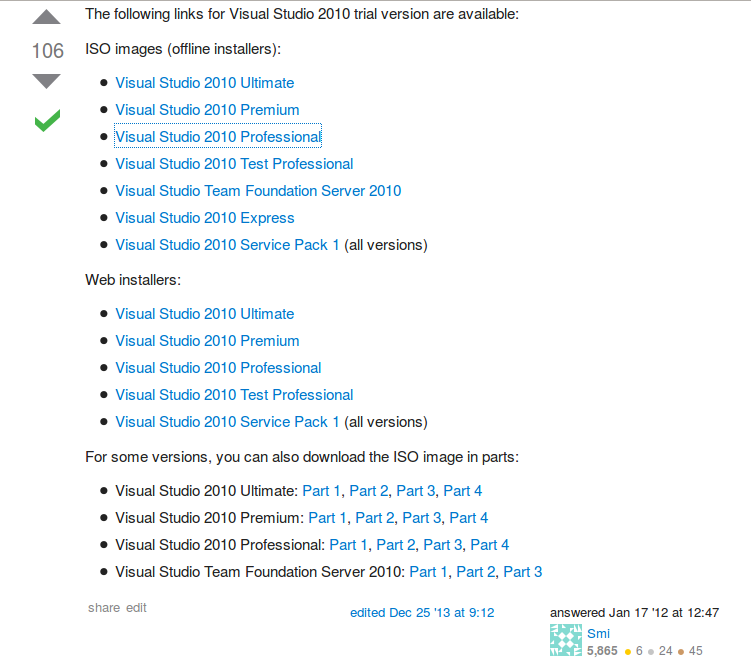
\includegraphics[scale=0.3]{step_0}
    \end{figure}
\end{frame}

\begin{frame}
    \frametitle{Downloading Setup Files}
    Step \# 2: Once it's downloaded, mount the image as a virtual drive. Windows 7 users might need to download and install \href{http://www.poweriso.com/download.php}{PowerISO} for `Mount' option to appear in the menu.
    \begin{figure}
        \centering
        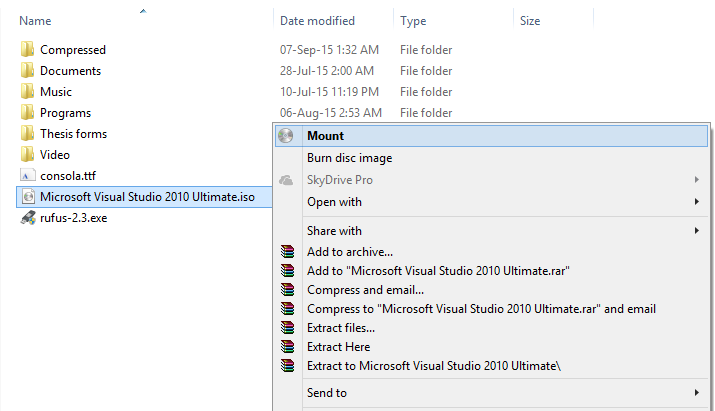
\includegraphics[scale=0.52]{step_0_1}
    \end{figure}
\end{frame}

\begin{frame}
    \frametitle{Installing the IDE}
    \subsection{Installing the IDE} % (fold)
    \label{sub:installing_the_ide}
    Step \# 1: Now, open the mounted/virtual drive and double-click the setup.exe file.
    \begin{figure}
        \centering
        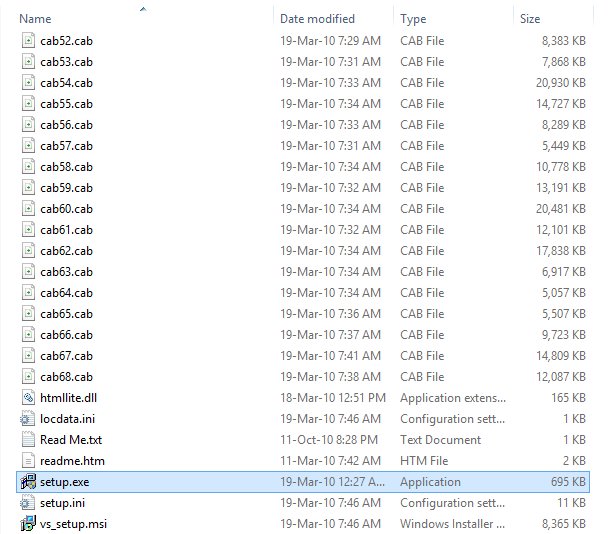
\includegraphics[scale=0.42]{step_0_2}
    \end{figure}
\end{frame}

\begin{frame}
    \frametitle{Installing the IDE}
    Step \# 2: In the window that appears, click `Install Microsoft Visual Studio 2010'.
    \begin{figure}
        \centering
        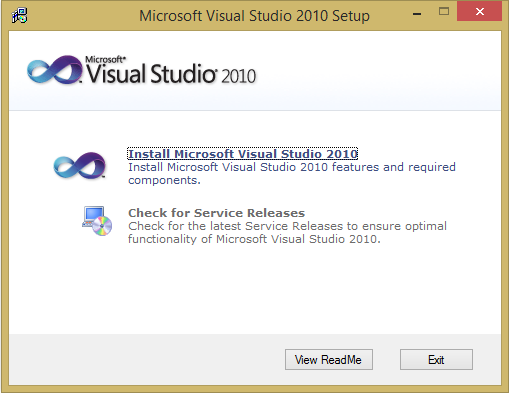
\includegraphics[scale=0.55]{step_1}
    \end{figure}
\end{frame}

\begin{frame}
    \frametitle{Installing the IDE}
    Step \# 3: Or you can choose to keep the check-box checked. Click `Next' to continue.
    \begin{figure}
        \centering
        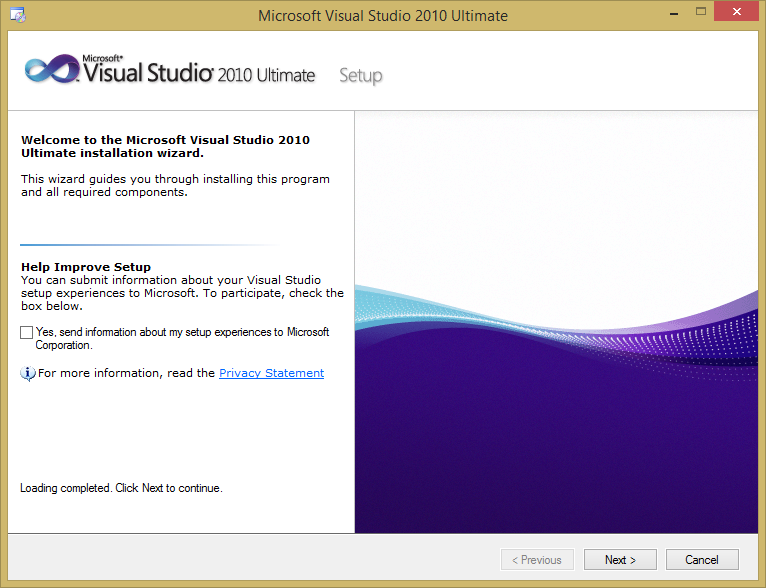
\includegraphics[scale=0.39]{step_2}
    \end{figure}
\end{frame}

\begin{frame}
    \frametitle{Installing the IDE}
    Step \# 4: This window notifies you of any pre-installed dependencies and presents Microsoft's license terms. Click the radio-button corresponding to `I have read and accept...' and click `Next' to continue.
    \begin{figure}
        \centering
        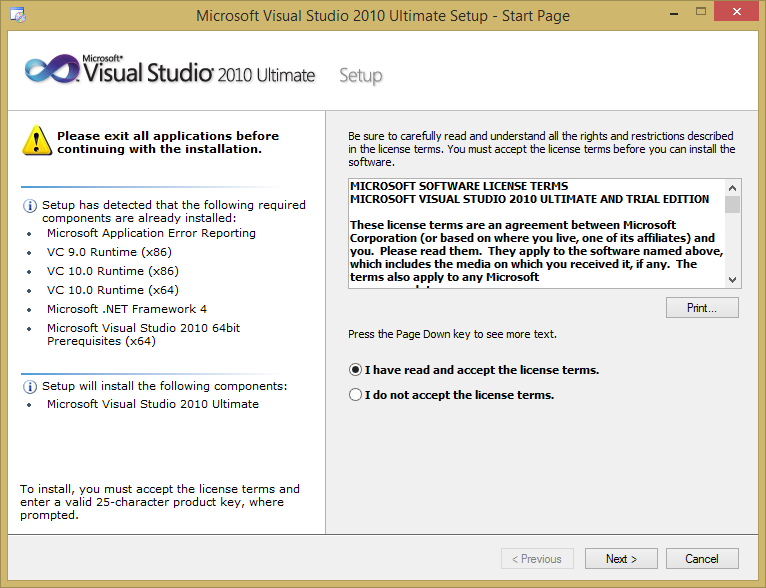
\includegraphics[scale=0.39]{step_3}
    \end{figure}
\end{frame}

\begin{frame}
    \frametitle{Installing the IDE}
    Step \# 5: 6.4 GB does not look like a lot of space to spare given the feature description and the fact that we want to use this IDE for our future projects too.
    \begin{figure}
        \centering
        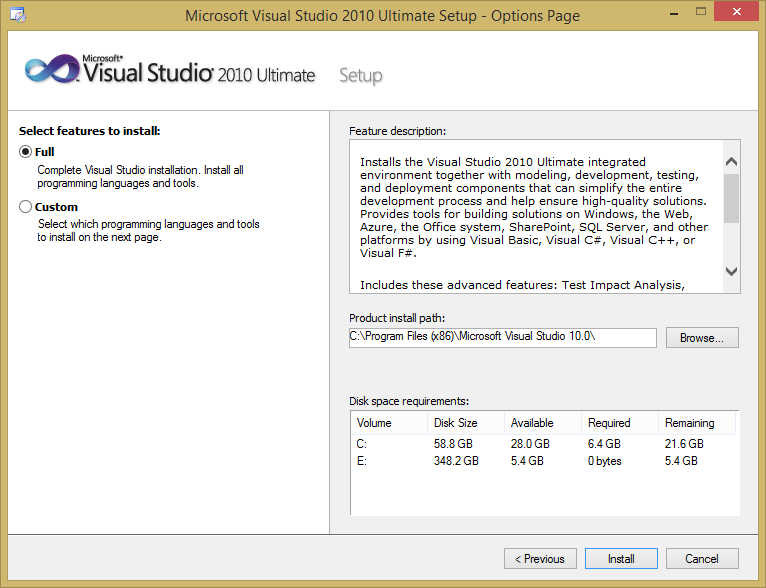
\includegraphics[scale=0.39]{step_4}
    \end{figure}
\end{frame}

\begin{frame}
    \frametitle{Installing the IDE}
    Step \# 6: If everything goes as expected, you will see a window much like this one with a progress bar and a few details related to components being installed.
    \begin{figure}
        \centering
        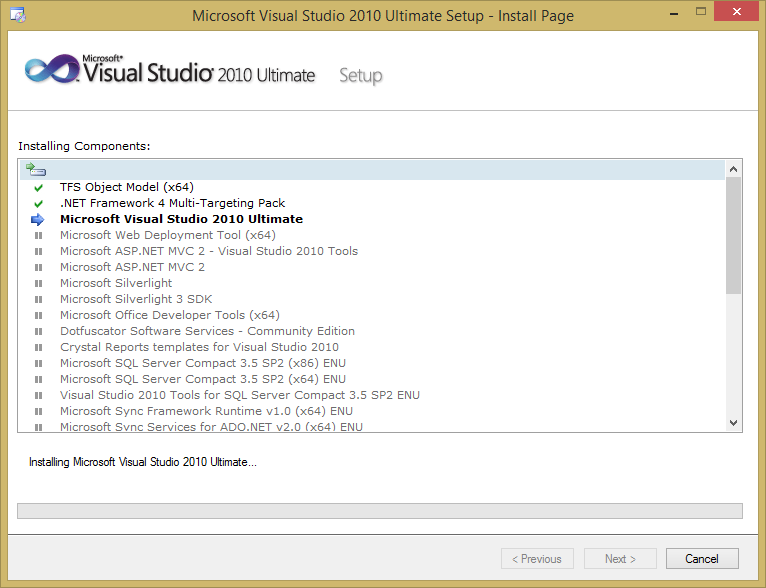
\includegraphics[scale=0.39]{step_5}
    \end{figure}
\end{frame}

\begin{frame}
    \frametitle{Installing the IDE}
    Step \# 7: ``Patience is bitter, but its fruit is sweet.'' -- Aristotle \\
    Click `Finish' and you are all set to create your first project.
    \begin{figure}
        \centering
        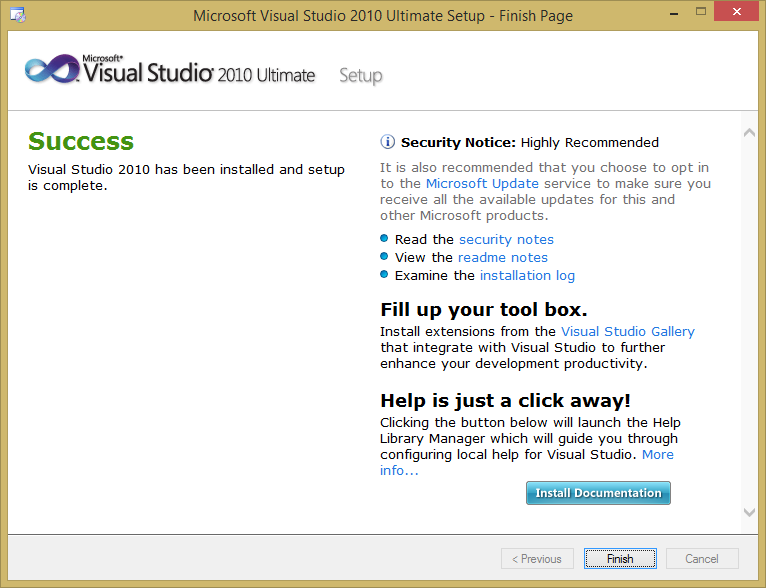
\includegraphics[scale=0.39]{step_6}
    \end{figure}
\end{frame}

\begin{frame}
    \frametitle{My First Project}
    \section{My First Project} % (fold)
    \label{sec:section_name}
    \subsection{Creating a New Project} % (fold)
    \label{sub:subsection_name}
    Step \# 1: Time to do something useful! Let's fire-up the IDE and create our first project. Wait! Before we do that, let's first set the default environment settings to those of `Visual C++'.
    \begin{figure}
        \centering
        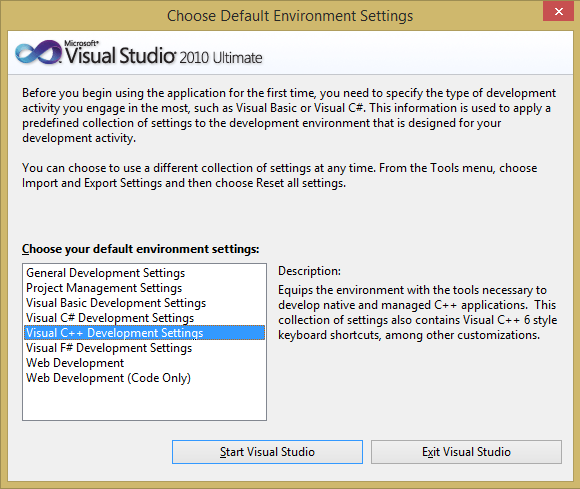
\includegraphics[scale=0.35]{step_7}
    \end{figure}
\end{frame}

\begin{frame}
    \frametitle{My First Project}
    Step \# 2: Click `New Project...' on the Start Page, `Open Project...' is used to access an existing project.
    \begin{figure}
        \centering
        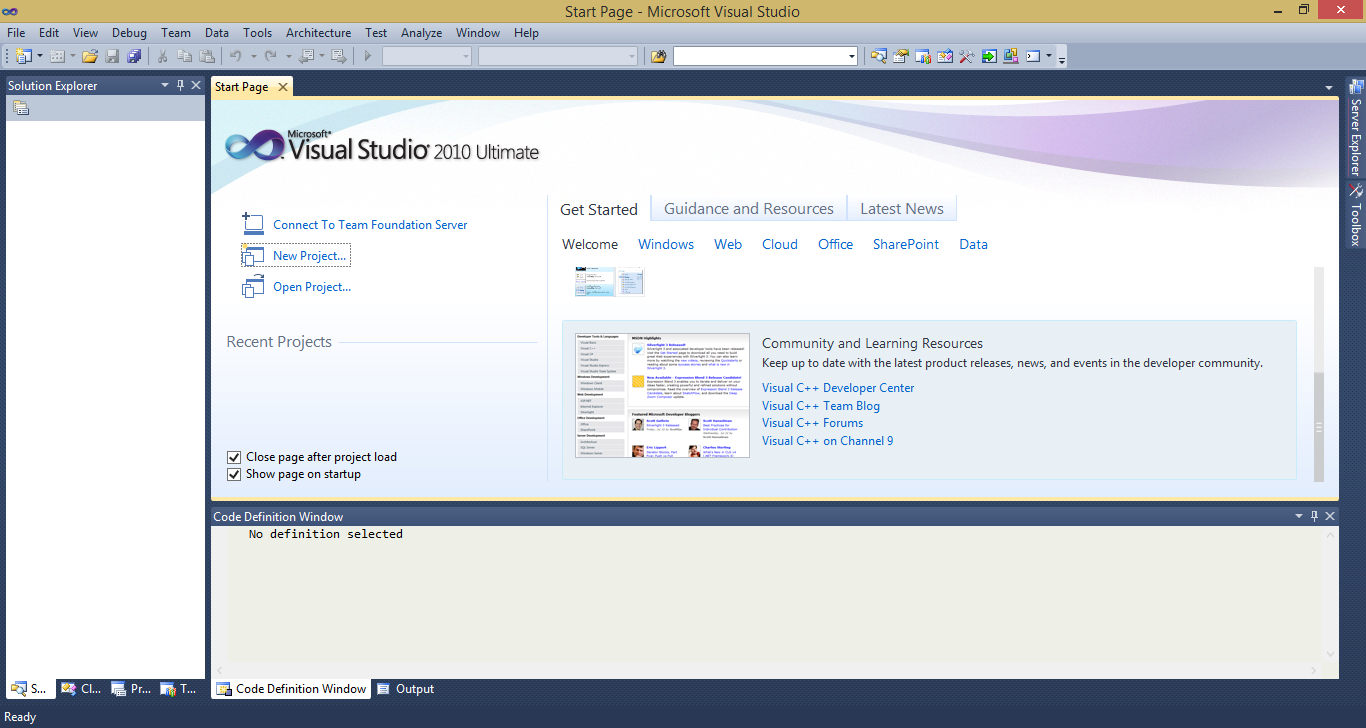
\includegraphics[scale=0.33]{step_8}
    \end{figure}
\end{frame}

\begin{frame}
    \frametitle{My First Project}
    Step \# 3: Select `Visual C++' in the `Installed Templates', and then `Empty Project' in the corresponding menu. Name the project, and if you don't want to save this project in the default location, use `Browse' select one of your own choice. Once you have done that, click `OK' to continue.
    \begin{figure}
        \centering
        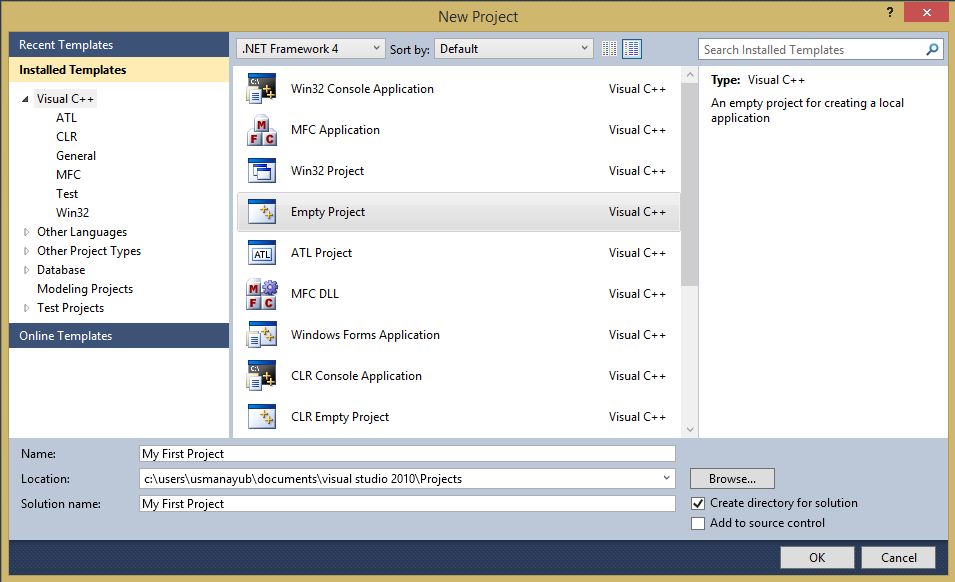
\includegraphics[scale=0.35]{step_9}
    \end{figure}
\end{frame}

\begin{frame}
    \frametitle{My First Project}
    \subsection{Adding Files to the Project} % (fold)
    \label{sub:adding_files}
    Step \# 4: Let's add something useful to this project. Right click on the project's name in the `Solution Explorer', hover over `Add' and click the `New Item' in the menu that appears.
    \begin{figure}
        \centering
        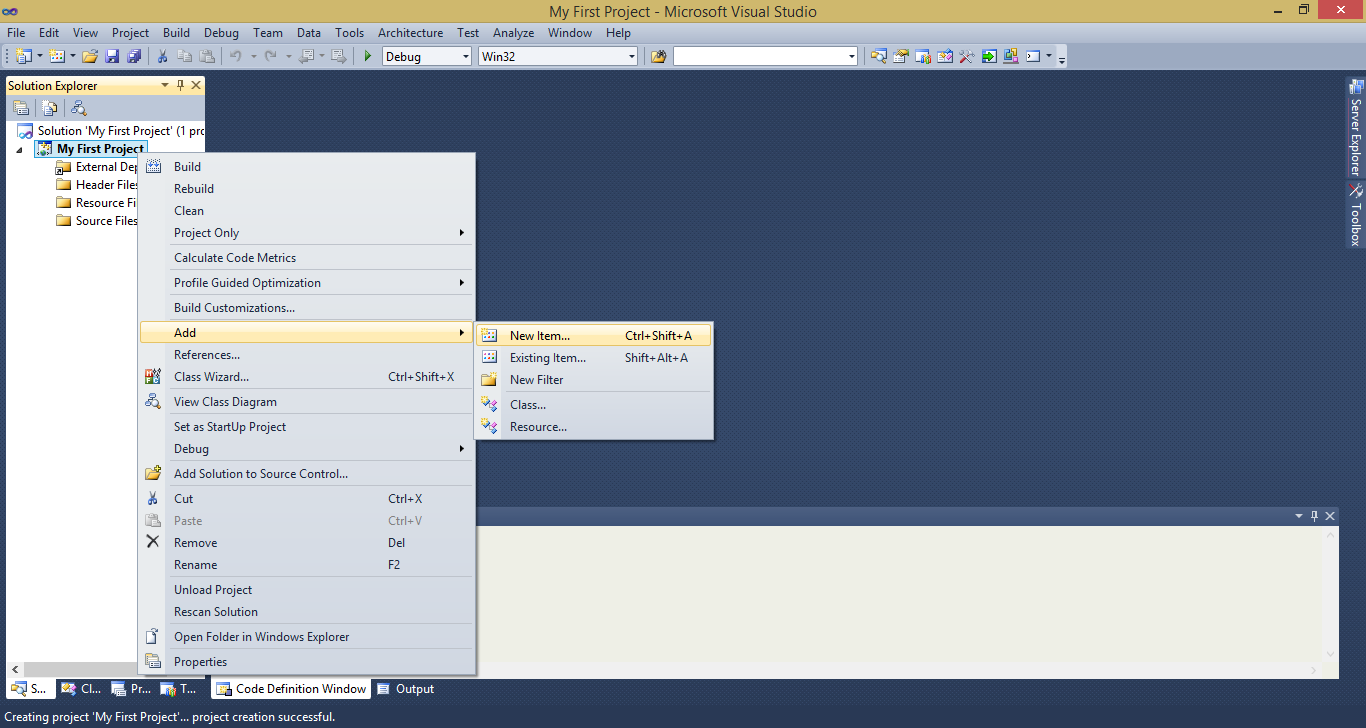
\includegraphics[scale=0.315]{step_10}
    \end{figure}
\end{frame}

\begin{frame}
    \frametitle{My First Project}
    Step \# 5: Select `C++ File (.cpp)', name the file and click `Add' to continue.
    \begin{figure}
        \centering
        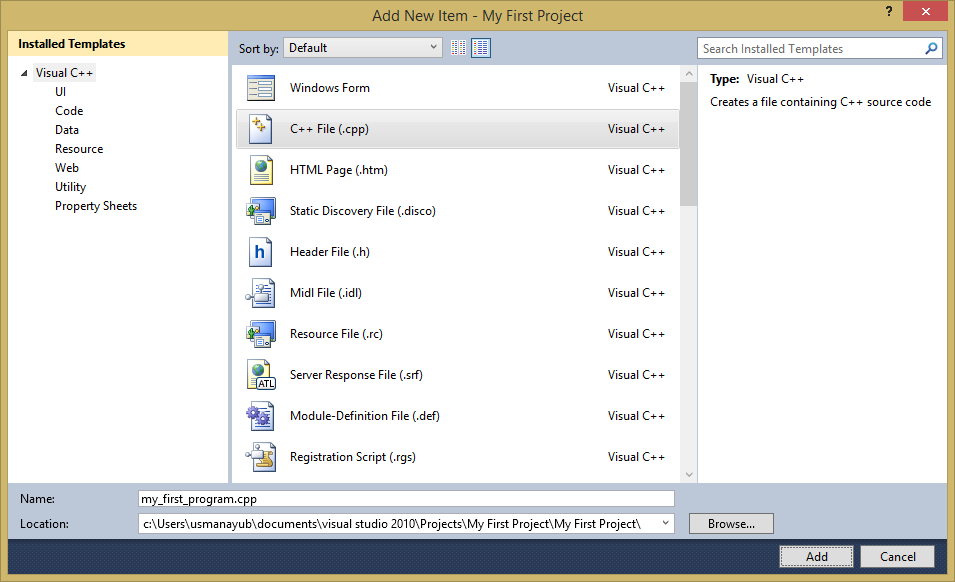
\includegraphics[scale=0.42]{step_11}
    \end{figure}
\end{frame}

\begin{frame}
    \frametitle{My First Project}
    Step \# 6: Now, a few other settings. By default, the `Line Numbers' are not enabled in the editor. To enable this feature, you'll need to go to `Tools' in the main menu and select `Options'.
    \begin{figure}
        \centering
        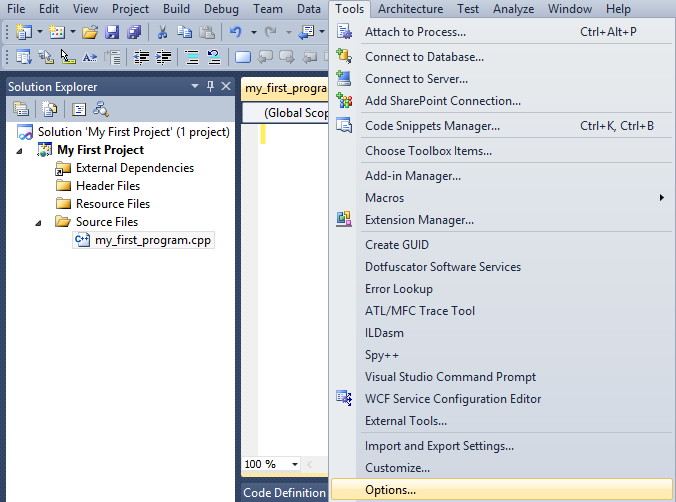
\includegraphics[scale=0.42]{step_12}
    \end{figure}
\end{frame}

\begin{frame}
    \frametitle{My First Project}
    Step \# 7: In the side bar of the window that appears, you'll need to expand the `Text Editor', expand `C/C++' from the sub-menu, select `General' from the sub-sub-menu and then check the box right next to `Line Numbers'.
    \begin{figure}
        \centering
        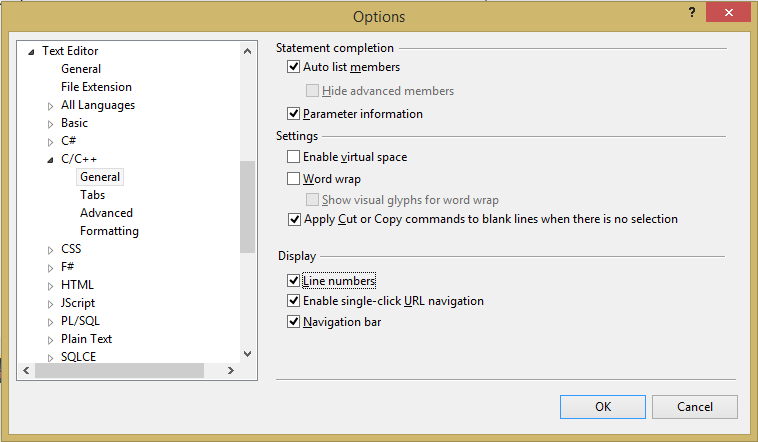
\includegraphics[scale=0.45]{step_13}
    \end{figure}
\end{frame}

\begin{frame}[fragile]
    \frametitle{My First Project}
    Step \# 8: Now that environment has been prepared, let's write our first program. Double-click the cpp file that you have created in Step 5 and start programming.
    \begin{lstlisting}[language=C++, basicstyle=\ttfamily,keywordstyle=\color{blue}]
    #include <iostream>
    using namespace std;
    int main()
    {
        cout << "This is my first program!";
        cout << endl;
        return 0;
    }\end{lstlisting}
\end{frame}

\begin{frame}
    \frametitle{My First Project}
    Step \# 9: In order to run this program, select `Start Without Debugging' in the `Debug' menu or use the short-cut \tt{CTRL + F5}.
    \begin{figure}
        \centering
        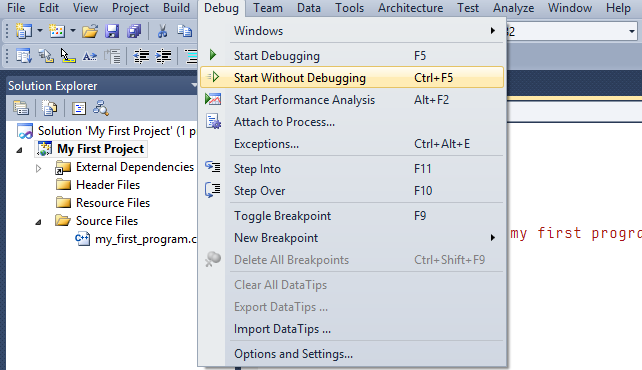
\includegraphics[scale=0.45]{step_14}
    \end{figure}
\end{frame}

\begin{frame}
    \frametitle{My First Project}
    Step \# 10: There you go, there's the output of your first program. Congratulations!
    \begin{figure}
        \centering
        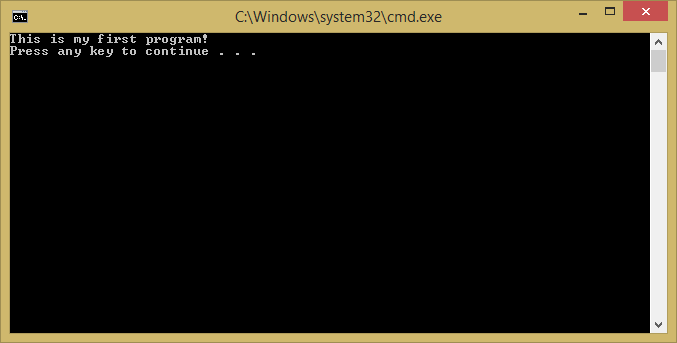
\includegraphics[scale=0.6]{step_15}
    \end{figure}
\end{frame}

\begin{frame}
    \frametitle{My First Project}
    Now let's play with this program a little bit. Let's remove different parts of it to see what happens, what error messages appear if we remove a semi-colon, let's add a few chunks to it and expand it's functionality somehow.
\end{frame}

\end{document}


